\documentclass[12pt]{article}
\usepackage{amsmath}
\usepackage{array}
% \usepackage{gensymb}
\usepackage{geometry}
\usepackage{graphicx}
\usepackage{pgfplots}
\usepackage{siunitx}
\usepackage{wrapfig}

\title{Homework \#11}
\author{Donald Aingworth IV}
\date{November 6, 2024}

\pgfplotsset{width=8cm,compat=1.9}
\usepgfplotslibrary{external}
% \tikzexternalize

\begin{document}

\DeclareSIUnit{\mile}{mi}
\DeclareSIUnit{\gal}{gal}
\DeclareSIUnit{\foot}{ft}
\DeclareSIUnit{\h}{h}

\maketitle

\pagebreak
\section*{Problem 1}
A neutron at rest decays into a proton, an electron, and a neutrino. If the proton's momentum is $3.00\times10^{-24}$ kg m/s in the direction 37\unit{\degree} N of E and the electron's momentum is $4.00\times10^{-24}$ kg m/s in the direction 53\unit{\degree} S of W, what is the momentum of the neutrino?

\subsection*{Solution}
We can first convert the angles. 
\[ 37\unit{\degree} \text{N of E} \rightarrow \theta_1 = 37\unit{\degree} \]
\[ 53\unit{\degree} \text{S of W} \rightarrow \theta_2 = 53\unit{\degree} + 180\unit{\degree} = 233\unit{\degree} \]

Now we can use the angles and momentum to calculate the sum of the two and then the resultant.
\begin{align*}
    p_+ &=  3.00\times10^{-24} \unit{\kilo\gram*\meter/\second} \begin{pmatrix} \cos(37\unit{\degree}) \\ \sin(37\unit{\degree}) \end{pmatrix}
        =   \begin{pmatrix} 3.00\times10^{-24}\cos(37\unit{\degree}) \\ 3.00\times10^{-24}\sin(37\unit{\degree}) \end{pmatrix} \unit{\kilo\gram*\meter/\second} \\
        &=  \begin{pmatrix} (3.00\times10^{-24}) * (7.986\times10^{-1}) \\ (3.00\times10^{-24}) * (6.018\times10^{-1}) \end{pmatrix} \unit{\kilo\gram*\meter/\second}
        =  \begin{pmatrix} 2.40\times10^{-24} \\ 1.81\times10^{-24} \end{pmatrix} \unit{\kilo\gram*\meter/\second}\\
    p_- &=  4.00\times10^{-24} \unit{\kilo\gram*\meter/\second} \begin{pmatrix} \cos(233\unit{\degree}) \\ \sin(233\unit{\degree}) \end{pmatrix}
        =   \begin{pmatrix} 3.00\times10^{-24}\cos(233\unit{\degree}) \\ 3.00\times10^{-24}\sin(233\unit{\degree}) \end{pmatrix} \unit{\kilo\gram*\meter/\second} \\
        &=  \begin{pmatrix} -2.41\times10^{-24} \\ -3.19\times10^{-24} \end{pmatrix} \unit{\kilo\gram*\meter/\second}\\
    p_\Sigma    &=  \begin{pmatrix} 2.40\times10^{-24} \\ 1.81\times10^{-24} \end{pmatrix} \unit{\kilo\gram*\meter/\second} + \begin{pmatrix} -2.41\times10^{-24} \\ -3.19\times10^{-24} \end{pmatrix} \unit{\kilo\gram*\meter/\second}\\
        &=  \begin{pmatrix} -1.14\times10^{-26} \\ -1.39\times10^{-24} \end{pmatrix} \unit{\kilo\gram*\meter/\second}\\
    &p_{neutrino}   =   \boxed{\begin{pmatrix} 1.14\times10^{-26} \\ 1.39\times10^{-24} \end{pmatrix} \unit{\kilo\gram*\meter/\second}}
\end{align*}

\pagebreak
\section*{Problem 2}
\begin{wrapfigure}{r}{0.35\textwidth}
    \vspace{-30pt}
    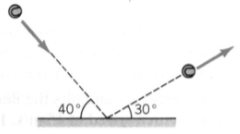
\includegraphics[width=0.35\textwidth]{graph_2.png} 
    % \label{fig:wrapfig}
\end{wrapfigure}
A 60.0-g tennis ball strikes the ground at 25.0 m/s at 40\unit{\degree} to the horizontal. It bounces off at 20.0 m/s at 30\unit{\degree} to the horizontal. (a) Find the impulse exerted on the ball. (b) If the collision lasted 5.00 ms, find the average force exerted on the ball by the court.

\subsection*{Solution}
\subsubsection*{Section (a)}
We use the formula for impulse, with the use of momentum.
\begin{align*}
    \vec{J} &=  \vec{p}_f - \vec{p}_i
        =   m*(\vec{v}_f - \vec{v}_i)
        =   0.06*\left( 20.0*\left(\begin{smallmatrix} \cos(30\unit{\degree}) \\ \sin(30\unit{\degree}) \end{smallmatrix}\right) - 25.0*\left(\begin{smallmatrix} \cos(-40\unit{\degree}) \\ \sin(-40\unit{\degree}) \end{smallmatrix}\right) \right) \unit{\kilo\gram\frac{\meter}{\second}}\\
        &=  0.06*\left( \begin{pmatrix} 17.32 \\ 10 \end{pmatrix} - \begin{pmatrix} 19.15 \\ -16.07 \end{pmatrix} \right) \unit{\kilo\gram\frac{\meter}{\second}}
        =   0.06*\begin{pmatrix} -1.8306 \\ 26.0697 \end{pmatrix} \unit{\kilo\gram\frac{\meter}{\second}}\\
        &=  \boxed{ \begin{pmatrix} -0.1098 \\ 1.5642 \end{pmatrix} \unit{\kilo\gram\frac{\meter}{\second}} }
\end{align*}

\subsubsection*{Section (b)}
Next, we use the formula for impulse from average force $\vec{J} = \vec{F}_{avg}\Delta t$.
\begin{align*}
    \vec{J} &=  \vec{F}_{avg}\Delta t\\
    \vec{F}_{avg}   &=  \frac{\vec{J}}{\Delta t}
        =   \frac{\begin{pmatrix} -0.1098 \\ 1.5642 \end{pmatrix} \unit{\kilo\gram\frac{\meter}{\second}}}{0.005 \unit{\second}}
        =   \boxed{ \begin{pmatrix} -21.967 \\ 312.836 \end{pmatrix} \unit{\newton} }
\end{align*}


\pagebreak
\section*{Problem 3}
A 1000-kg Subaru at rest at a stoplight is struck from the rear by a 1400-kg Pontiac. They couple together and leave skid marks 4.25 m long. The coefficient of kinetic friction is 0.6. (a) What was their common speed just after the collision? (b) What was the speed of the Pontiac just prior to the collision?

\subsection*{Solution}
We assume they travel the distance equivalent to the length of their skid marks. Together, the mass of the two-object system is 1000kg + 1400kg = 2400kg. 
\subsubsection*{Section (a)}
We can here start with the work done on an object and associated formulae.
\[ W = \Delta E_{mech} + \Delta E_{th} = \Delta K + \Delta U + \Delta E_{th} \]
Since this is no work added to the system after the collision, we have $W = 0$. We can use the conservation of energy to use further formulae. The potential energy also does not change because all the kinetic energy lost will be converted into friction, thermal energy.
\[ 0 = K_f - K_i + E_{th;f} - E_{th;i} = m*\left( \frac{1}{2}v_f^2 - \frac{1}{2}v_i^2 + g*d_f - g*d_i \right) \]
It starts at an initial position of zero and a final velocity of zero.
\begin{align*}
    0   &=  g*d_f - \frac{1}{2}v_i^2\\
    \frac{1}{2}v_i^2    &=  g*d_f\\
    v_i &=  \sqrt{2*\mu_k*g*d_f}
        =   \sqrt{2*0.6*9.81\unit{\meter/\second^2}*4.25\unit{\meter}}\\
        &=  \sqrt{5.10*9.81} \unit{\meter/\second}
        =   \sqrt{50.031}\unit{\meter/\second}
        =   \boxed{7.073\unit{\meter/\second}}
\end{align*}
\pagebreak
\subsubsection*{Section (b)}
We can use the conservation of momentum, keeping in mind that since $\vec{v}_{1;i} = 0$, then \(\vec{p}_{1;i} = 0\). We also keep in mind that after collision, the two cars travel at the same velocity.
\begin{align*}
    p_{1;i} + p_{2;i} &= p_{1;f} + p_{2;f}\\
    m_1*v_{1;i} &=  m_\Sigma * v_f\\
    v_{1;i} &=  \frac{m_\Sigma * v_f}{m_1}
\end{align*}
From this, we can plug in numbers to find the velocity before collision.
\begin{align*}
    v_{1;i} &=  \frac{m_\Sigma * v_f}{m_1}
        =   \frac{2400\unit{\kilo\gram} * 7.073\unit{\meter/\second}}{1400\unit{\kilo\gram}}
        =   \boxed{\frac{12*\sqrt{50.031}}{7}\unit{\meter/\second} 
        =   12.126\unit{\meter/\second}}
\end{align*}


\pagebreak
\section*{Problem 4}
Two particles with masses $m_1$ and $m_2$ travel toward each other with velocities $v_{1,i}$ and $v_{2,i}$. They collide and stick together. Show that the loss in kinetic energy is
\[ \frac{m_1 m_2 \left(v_{1,i} - v_{2,i}\right)^2}{2(m_1 + m_2)} \]

\subsection*{Solution}
We first can calculate the velocity after collision by using the conservation of momentum. We also keep in mind that they stick together afterwards and the fact that particle 2 has negative velocity in this instance.
\begin{align*}
    p_{1,i} + p_{2,i} &=  p_{1,f} + p_{2,f}\\
    m_1 v_{1,i} - m_2 v_{2,i} &=  (m_1 + m_2) v_f\\
    v_f &=  \frac{m_1 v_{1,i} - m_2 v_{2,i}}{m_1 + m_2}
\end{align*}

We then use the formulae \( \Delta K = K_f - K_i \) and \( K = \frac{1}{2}mv^2 \).
\begin{align*}
    \Delta K &= K_f - K_i
        =   K_f - (K_{1,i} + K_{2,i})
        =   \frac{1}{2}m_\Sigma v_f^2 - \left(\frac{1}{2}m_1v_{1,i}^2 + \frac{1}{2}m_2v_{2,i}^2\right)\\
        &=  \frac{1}{2}\left( (m_1 + m_2) \left(\frac{m_1 v_{1,i} - m_2 v_{2,i}}{m_1 + m_2}\right)^2 - m_1v_{1,i}^2 - m_2v_{2,i}^2 \right)\\
        &=  \frac{(m_1 v_{1,i} - m_2 v_{2,i})^2}{2(m_1 + m_2)} - \frac{m_1v_{1,i}^2 + m_2v_{2,i}^2}{2}\\
        &=  \frac{m_1^2 v_{1,i}^2 - 2m_1m_2v_{1,i}v_{2,i} + m_2^2 v_{2,i}^2}{2(m_1 + m_2)} - \frac{m_1^2v_{1,i}^2 + m_1m_2v_{1,i}^2 + m_1m_2v_{2,i}^2 + m_2^2v_{2,i}^2}{2(m_1 + m_2)}\\
        &=  -\frac{m_1m_2v_{1,i}^2 + 2m_1m_2v_{1,i}v_{2,i} + m_1m_2v_{2,i}^2}{2(m_1 + m_2)}\\
        &=  -\frac{m_1m_2(v_{1,i}^2 + 2v_{1,i}v_{2,i} + v_{2,i}^2)}{2(m_1 + m_2)}
        =   -\frac{m_1m_2(v_{1,i} + v_{2,i})^2}{2(m_1 + m_2)}
\end{align*}
Since this is a negative change, that means the kinetic energy is lost. In other words, the amount of kinetic energy lost is \boxed{\frac{m_1m_2(v_{1,i} + v_{2,i})^2}{2(m_1 + m_2)}}.

\pagebreak
\section*{Problem 5}
\begin{wrapfigure}{r}{0.35\textwidth}
    \vspace{-30pt}
    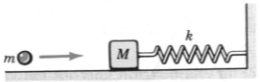
\includegraphics[width=0.35\textwidth]{graph_5.png} 
    % \label{fig:wrapfig}
\end{wrapfigure}
A projectile of mass 0.25 kg moving at 24.0 m/s collides with and sticks to a 1.75-kg block that is connected to a spring for which k = 40.0 N/m, as in the figure below. The block is initially on a frictionless part of a horizontal surface but starts to slide on a rough section immediately after the collision. If the maximum compression of the spring is 0.5 m, what is the force of friction on the block?

\subsection*{Solution}
First, we find the post-collision velocity \(v_c\) using the post-collision momentum \(p_c\).
\begin{align*}
    M   &=  m_1 + m_2
        =   0.25\unit{\kilo\gram} + 1.75\unit{\kilo\gram}
        =   2.00\unit{\kilo\gram}\\
    p_c &=  p_{1;i} + p_{2;i}\\
    Mv_c    &=   m_1 v_{1;i} + m_2 v_{2;i}\\
    v_c &=  \frac{m_1 v_{1;i}}{M}
\end{align*}

Next, we calculate the initial kinetic energy from that. 
\begin{equation*}
    K_i =   \frac{1}{2}Mv_f^2
        =   \frac{m_1^2 v_{1;i}^2}{2M}
\end{equation*}

With that, we can apply the conservation of energy, knowing that no work is applied on the system between the collision and when the block stops. Then we apply zeroes where necessary for formulae containing zeroes.
\begin{align*}
    K_f + U_f   + E_{th;f}    &=  K_i + U_i + E_{th;i}\\
    0   + \frac{1}{2}kx^2   +   f_k x   &=  \frac{1}{2}Mv_c^2 + 0 + 0
\end{align*}

Now, we can solve for $f_k$, which is what we're looking for.
\begin{align*}
    \frac{1}{2}kx^2   +   f_k x   &=  \frac{1}{2}Mv_c^2\\
    f_k &=  \frac{Mv_c^2 - kx^2}{x}
        =   \frac{m_1^2 v_{1;i}^2}{2Mx} - \frac{1}{2}kx
\end{align*}

From this, we substitute in values.
\[ f_k = \frac{m_1^2 v_{1;i}^2}{2Mx} - \frac{1}{2}kx = \frac{0.25^2 24.0^2}{2*2*0.5}\unit{\newton} - \frac{1}{2}40*0.5 \unit{\newton} = \boxed{8\unit{\newton}} \]


\pagebreak
\section*{Problem 6}
\begin{wrapfigure}{r}{0.35\textwidth}
    \vspace{-58pt}
    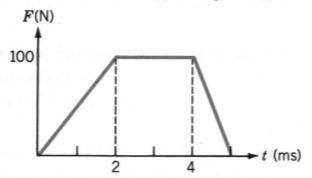
\includegraphics[width=0.35\textwidth]{graph_6.png} 
    % \label{fig:wrapfig}
\end{wrapfigure}
From the F versus t curve shown to the right, find: (a) the impulse; (b) the average force.

\subsection*{Solution}
\subsubsection*{Section (a)}
Impulse (J) is equal to the integral of the force with respect to time. This is equivalent to the area under the curve. We also convert milliseconds to seconds.
\begin{align*}
    J   &=  \int_{0}^{0.005} F(t)\ dt
        =   \int_{0}^{0.002} F(t)\ dt + \int_{0.002}^{0.004} F(t)\ dt + \int_{0.004}^{0.005} F(t)\ dt\\
        &=  \frac{1}{2}*100*0.002 \unit{\kilo\gram*\meter/\second} + 100*0.002 \unit{\kilo\gram*\meter/\second} + \frac{1}{2}100*0.001 \unit{\kilo\gram*\meter/\second}\\
        &=  0.1 \unit{\kilo\gram*\meter/\second} + 0.2 \unit{\kilo\gram*\meter/\second} + 0.05 \unit{\kilo\gram*\meter/\second}
        =   \boxed{0.35 \unit{\kilo\gram*\meter/\second}}
\end{align*}

\subsubsection*{Section (b)}
We know that \( J = F_{avg}\Delta t \), which we can manipulate to find the average force. We already know the impulse from above.
\begin{align*}
    F_{avg} &=  \frac{J}{\Delta t}
        =   \frac{0.35 \unit{\kilo\gram*\meter/\second}}{0.005 \unit{\second}}
        =   \frac{350}{5}\unit{\newton}
        =   \boxed{ 70\unit{\newton} }
\end{align*}

\pagebreak
\section*{Problem 7}
A nucleus of radioactive radium ($^{226}$Ra), initially at rest, decays into a radon nucleus ($^{222}$Rn) and an $\alpha$-particle (a $^{4}$He nucleus). If the kinetic energy of the $\alpha$-particle is $6.72 \times 10^{-13}$ J, what is (a) the recoil speed of the radon nucleus, and (b) its kinetic energy? The superscripts indicate, roughly, the mass of each nucleus in unified mass units (u), where 1 u = $1.66 \times 10^{-27}$ kg.

\subsection*{Solution}
I'm not a chemist, to be honest. Still, I'll try to do this with Physics only. To find the mass of each object, we have to convert the atomic mass into mass.
\begin{align*}
    \text{Radium: }&    226 * 1.66\times 10^{-27}\unit{\kilo\gram} = 3.7516\times 10^{-25}\unit{\kilo\gram}\\
    \text{Radon: }&    222 * 1.66\times 10^{-27}\unit{\kilo\gram} = 3.6852\times 10^{-25}\unit{\kilo\gram}\\
    \alpha\text{-particle: }&    4 * 1.66\times 10^{-27}\unit{\kilo\gram} = 6.64\times 10^{-27}\unit{\kilo\gram}
\end{align*}

\subsubsection*{Section (a)}
To get the velocity of the $\alpha$-particles from the kinetic energy, we use this.
\begin{equation*}
    K   =   \frac{1}{2}mv^2\rightarrow
    v   =   \sqrt{\frac{2K}{m}} 
        =   \sqrt{\frac{1.344 \times 10^{-12}\unit{\joule}}{6.64\times 10^{-27}\unit{\kilo\gram}}}
        =   1.4227\times10^7 \unit{\meter/\second}
\end{equation*}
Since the velocity (and momentum) starts at zero, and the objects go in opposite directions, we can write \(m_1v_1 = m_2v_2\).
\begin{align*}
    m_1v_1  &= m_2v_2\\
    v_1 &=  \frac{m_2v_2}{m_1}
        =   \frac{6.64\times 10^{-27}\unit{\kilo\gram} * 1.4227\times10^7 \unit{\meter/\second}}{3.6852\times 10^{-25}\unit{\kilo\gram}}
        =   \boxed{2.563\times10^5 \unit{\meter/\second}}
\end{align*}

\subsubsection*{Section (b)}
Here, we use the formula for kinetic energy.
\begin{align*}
    K   &=  \frac{1}{2}mv^2
        =   \frac{1}{2}(3.6852\times 10^{-25}\unit{\kilo\gram})(2.563\times10^5 \unit{\meter/\second})^2
        =   \boxed{1.2108\times10^{-14} \unit{\joule}}
\end{align*}


\pagebreak
\section*{Problem 8}
\begin{wrapfigure}{r}{0.35\textwidth}
    \vspace{-30pt}
    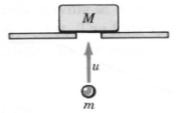
\includegraphics[width=0.35\textwidth]{graph_8.png} 
    % \label{fig:wrapfig}
\end{wrapfigure}
A projectile of mass $m$ = 200 g strikes a stationary block of mass $M$ = 1.30 kg from below with speed $u$ = 30.0 m/s as shown in the figure below. The projectile embeds in the block. (a) To what height does the block rise? (b) What is the loss in kinetic energy due to the collision?

\subsection*{Solution}
\subsubsection*{Section (a)}
We start by recalling the conservation of linear momentum.
\[ \vec{p}_{1i} + \vec{p}_{2i} = \vec{p}_{1f} + \vec{p}_{2f} \]
\[ m_1\vec{v}_{1i} + m_2\vec{v}_{2i} = m_1\vec{v}_{1f} + m_2\vec{v}_{2f} \]

Keeping in mind that the initial velocity will be zero for the block ($m_2$) and the post-collision velocity will be identical for both blocks, we apply the above formula to get the post-collision velocity for the whole system.
\begin{align*}
    m_1\vec{v}_{1i} &=  (m_1 + m_2)\vec{v}_{f}\\
    \vec{v}_{f} &=  \frac{m_1\vec{v}_{1i}}{m_1 + m_2} = \frac{m*u}{m+M}
\end{align*}

Next, we can use this to find the post-collision initial kinetic energy, then use the conservation of mechanical energy to determine the potential energy once the kinetic energy (and the velocity) is zero.
\begin{align*}
    K_i &=  \frac{1}{2}mv^2
        =   \frac{1}{2}(m+M)\left(\frac{m*u}{m+M}\right)^2
        =   \frac{m^2*u^2}{2(m+M)}\\
    U_g &=  K_i\rightarrow
    (m+M)*g*\Delta y    =  \frac{m^2*u^2}{2(m+M)}\\
    \Delta y    &=  \frac{m^2*u^2}{2g(m+M)^2}
        =   \frac{0.20^2*30.0^2}{2*9.81(0.20+1.30)^2}\unit{\meter}
        =   \frac{36}{19.62*2.25}\unit{\meter}
        =   \boxed{0.815\unit{\meter}}
\end{align*}

\pagebreak
\subsubsection*{Section (b)}
Here the formula is \( \Delta K = K_f - K_i \). We can calculate the initial kinetic energy and from that the change in kinetic energy. We can keep in mind that what in part (a) would be called \(K_i\) in this instance is \(K_f\) to rewrite our equation.
\begin{align*}
    \Delta K    &=  K_f - K_i
        =   \frac{m^2*u^2}{2(m+M)} - \frac{1}{2}mu^2
        =   \frac{1}{2}mu^2\left(\frac{m}{m+M} - 1\right)\\
        &=  0.10*30^2\left(\frac{0.20}{0.20+1.30} - 1\right) \unit{\joule}
        =   90\left(\frac{2.00}{15.00} - 1\right) \unit{\joule}\\
        &=  \boxed{-\frac{1170}{15} \unit{\joule} = -78.0 \unit{\joule}}
        % =   \frac{m^3*u^2}{2(m+M)^2} - \frac{1}{2}mu^2
        % =   \frac{1}{2}mu^2\left(\frac{m^2}{(m+M)^2} - 1\right)\\
        % &=  0.10*30^2\left(\frac{0.20^2}{(0.20+1.50)^2} - 1\right) \unit{\joule}
        % =   90\left(\frac{4.00}{289.00} - 1\right) \unit{\joule}\\
        % &=  \boxed{-\frac{25650}{289} \unit{\joule} = -88.754 \unit{\joule}}
\end{align*}

\end{document}